\section{Einleitung}
\subsection{Einführung in die Thematik}
\blindtext\nomenclature{W3C}{World Wide Web Consortium}
\blindtext\footcite[Vgl. ][]{mswpf}

\subsection{Problemstellung und Zielsetzung}
\blindtext

\subsection{Methodischer Aufbau der Arbeit}
\blindtext

\section{Hauptteil}
\subsection{Grundlagen der Wirtschaftsinformatik}
\blindtext (vgl. Abbildung \ref{abb_bsp}).\footcite[Vgl. ][]{msdatabind}\footcite[Vgl. ][]{Atypisch}\footcite[Vgl. ][34]{Digitaloekonomie}
\blindenumerate
\Blindtext

\begin{figure}[!htb]
    \caption{Terminal}
    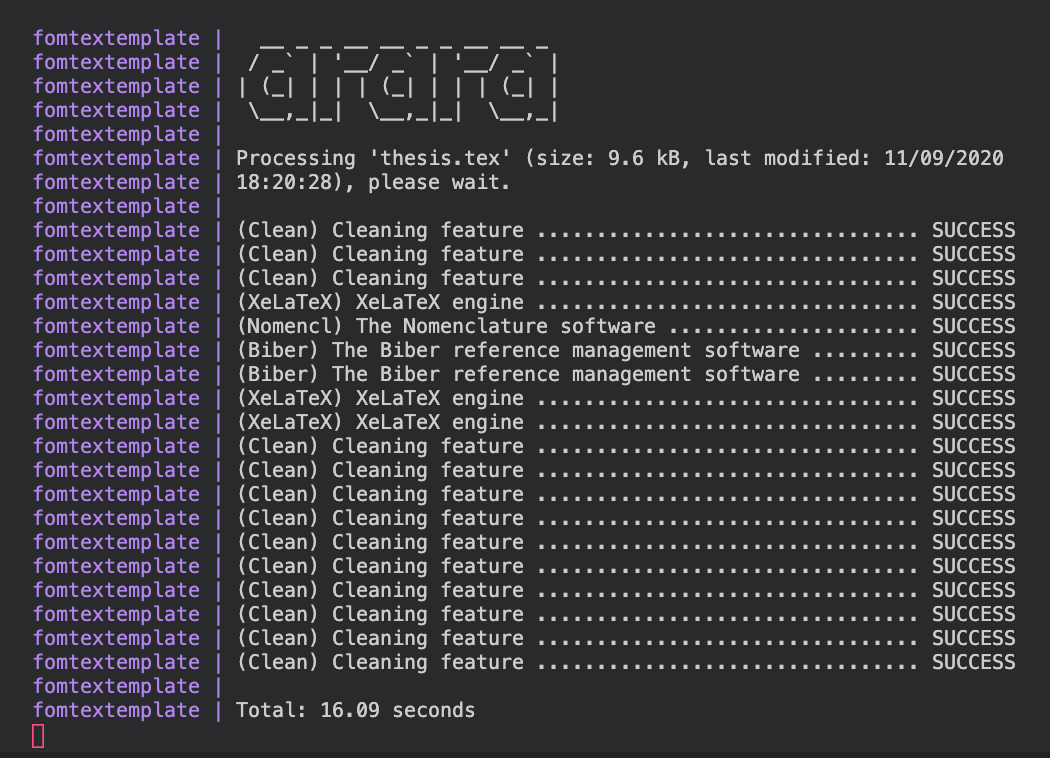
\includegraphics[width=1\textwidth]{.github/terminal}
    \captionsetup{width=1\textwidth}
    \capquelle{\cite[][200]{bsp}}\label{abb_bsp}
\end{figure}
\blindtext\footcite[Vgl. ][415-426]{Tanenbaum2016}

\subsubsection{Design-Prinzip der Separierung von Verantwortlichkeiten}
\blindtext\footcite[Vgl. ][79]{Schelinski2019}
\blinditemize\footcite[Vgl. ][34]{Digitaloekonomie}
\Blindtext

\begin{tabular}{cccc}
    Material        & Symbol &  eg  & Type \\
    \hline
    diamond         & C      & 5.46 & i \\
    silicon         & Si     & 1.12 & i \\
    germanium       & Ge     & 0.67 & i \\
    selenium        & Se     & 1.74 & d \\
    \hline
    \captionsetup{width=.7\textwidth}
    \capquelle{\cite[][212]{bsp}}\label{tab_bsp}
\end{tabular}

\section{Schluss}
\subsection{Fazit}
\Blindtext






